%picdispkurve,picapparatur,picsymstrahl,picprismawinkel,picbrechwinkel
%eqbrech, eqdispcurve, eqdisp1, eqdisp2
\subsection{Brechung und Dispersion}
	\begin{figure}[h]
		\begin{center}
		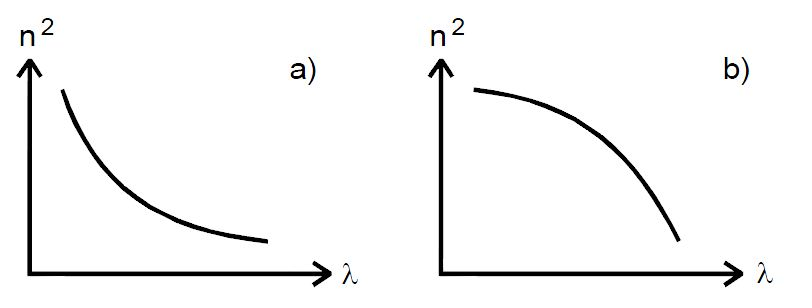
\includegraphics[scale=0.7]{picdispkurve.jpg}
		\caption{Gestalt möglicher Dispersionskurven[1]}
		\label{picdispkurve}
		\end{center}	
	\end{figure}
Durch Wechselwirkungen mit Elektronen ist die Geschwindigkeit von Licht in Materie
geringer als die Vakuumslichtgeschwindigkeit. Dadurch kommt es zu Brechungen an 
Materiegrenzflächen nach Gleichung (\ref{eqbrech}) mit dem Brechungsindex $n$.
Da die Ausbreitungsgeschwindigkeit von der Wellenlänge $\lambda$ des Lichtes abhängt, 
wird Licht unterschiedlicher Frequenz verschieden stark gebrochen. Dieses
Phänomen wird Dispersion genannt. Eine Abhängigkeit nach (\ref{eqdispkurve})
heißt Dispersionskurve\cite{anleitung} (vgl. Abb. \ref{picdispkurve}).
\begin{align}
n&=\frac{v_1}{v_2} \label{eqbrech} \\
v_1&, v_2 : \text{materialabhängige Geschwindigkeit von Licht} \nonumber \\
n&=f(\lambda) \label{eqdispkurve}
\end{align}
Aus dem Huygensschen Prinzip lässt sich das Snelliussche Brechungsgesetz (Gl. (\ref{eqsnellius})) folgern,
bei einem Eintritt unter einem Winkel $\alpha$ folgt mit dem Brechungsindex $n$ ein
Austrittswinkel $\beta$.
\begin{align}
n&=\frac{sin \alpha}{sin \beta}\label{eqsnellius}
\end{align}
\subsection{Dispersion an einem Prisma}
Unter Annahme eines Strahlendurchgangs von sichtbarem Licht von Luft in
ein durchsichtiges, farbloses Material lassen sich Dispersionsgleichungen \cite{anleitung} ableiten:
Gilt für die Absorbtionsstelle $\lambda_1$ mit der Wellenlänge $\lambda$ im Vakuum, dass $\lambda>>\lambda_1$,
so gilt Gleichung (\ref{eqdisp1}), welche in Abbildung \ref{picdispkurve} als a) dargestellt ist.
Gilt hingegen $\lambda<<\lambda_1$, so gilt Gleichung (\ref{eqdisp2}), welche in Abbildung \ref{picdispkurve} 
als b) dargestellt ist. Beide Kurven beschreiben normale Dispersion, also Abnahme von $n$ bei Zunahme von $\lambda$.
\begin{align}
n^2(\lambda)&=A_0+\frac{A_2}{\lambda^2}+\frac{A_4}{\lambda^4}+\ldots \text{ mit } A_i>0 \label{eqdisp1} \\
n^2(\lambda)&=1-A_2' \lambda^2-A_4'\lambda4-\ldots \text{ mit } A_i'>0, i\geq 2 \label{eqdisp2}
\end{align}
\subsection{Prismenspektralapparat}
	\begin{figure}[h]
		\begin{center}
		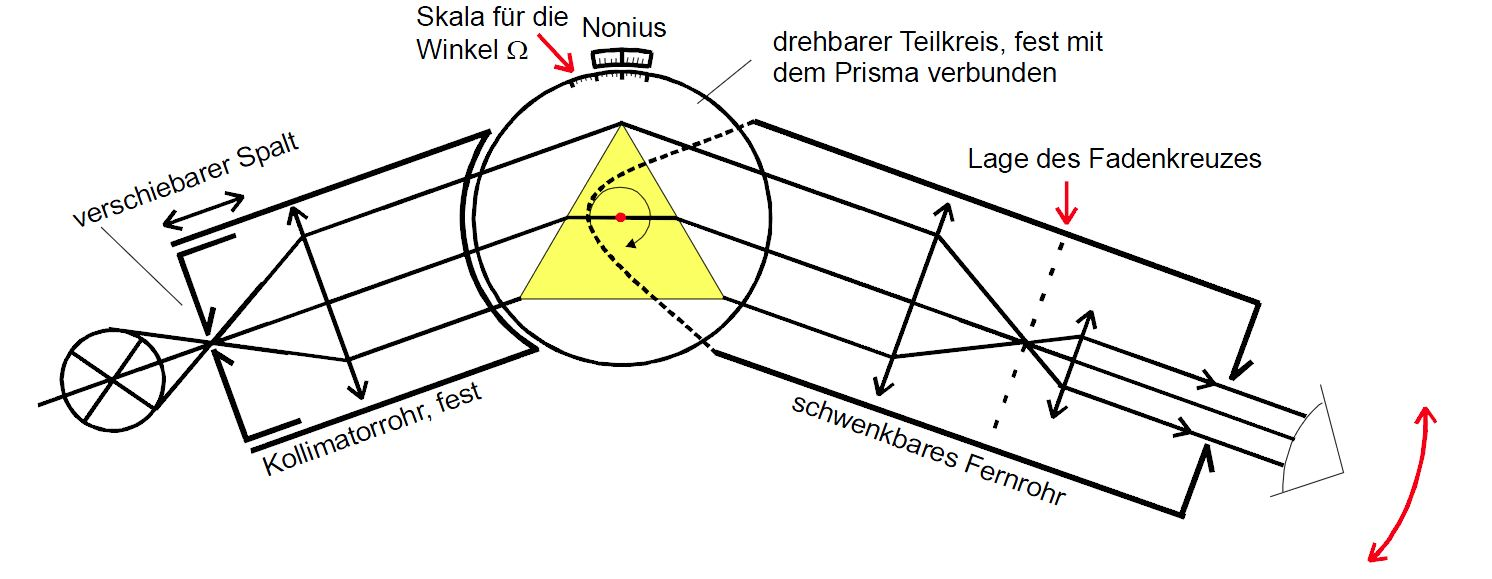
\includegraphics[scale=0.3]{picapparatur.jpg}
		\caption{Schematische Darstellung des Prismenspektralapparates[1]}
		\label{picapparatur}
		\end{center}	
	\end{figure} 	\begin{figure}[h]
		\begin{center}
		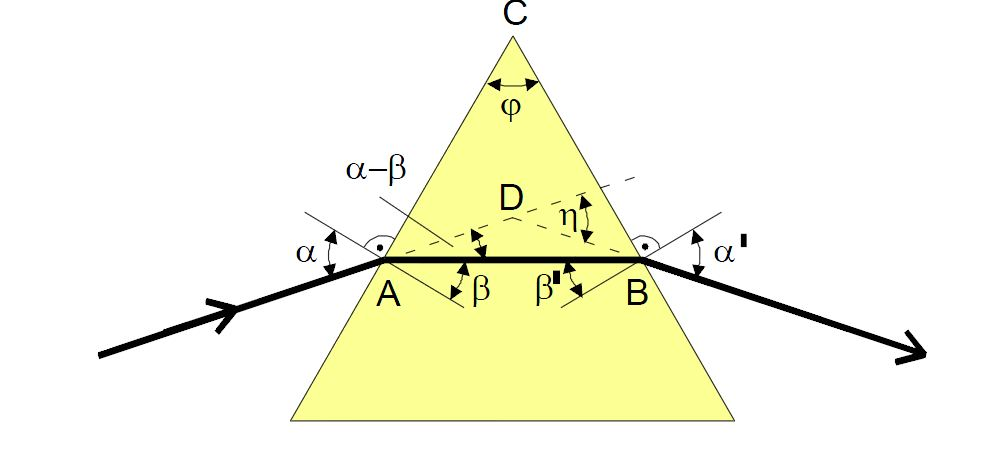
\includegraphics[scale=0.4]{picsymstrahl.jpg}
		\caption{Symmetrischer Strahlengang durch ein Prisma[1]}
		\label{picsymstrahl}
		\end{center}	
	\end{figure}
Mit Hilfe eines Prismenspektralapparates (siehe Abb. \ref{picapparatur}) lässt sich der Brechungsindex 
abhängig von der Wellenlänge durch ABlesen von Winkeln bestimmen. Das Gerät macht sich das Snelliussche Brechungsgesetz zu nutze,
bei dem symmetrischen Durchgang des Lichtstrahls (Abb. \ref{picsymstrahl}) lässt sich folgende Gleichung 
herleiten.
\begin{align}
n&=\frac{sin\frac{\eta + \phi}{2}}{\frac{\phi}{2}}\\
\text{ mit }\alpha&=\frac{\eta + \phi}{2}
\end{align}
\subsection{Bestimmung des Brechungswinkels zwischen brechenden Oberflächen des Prismas}
	\begin{figure}[h]
		\begin{center}
		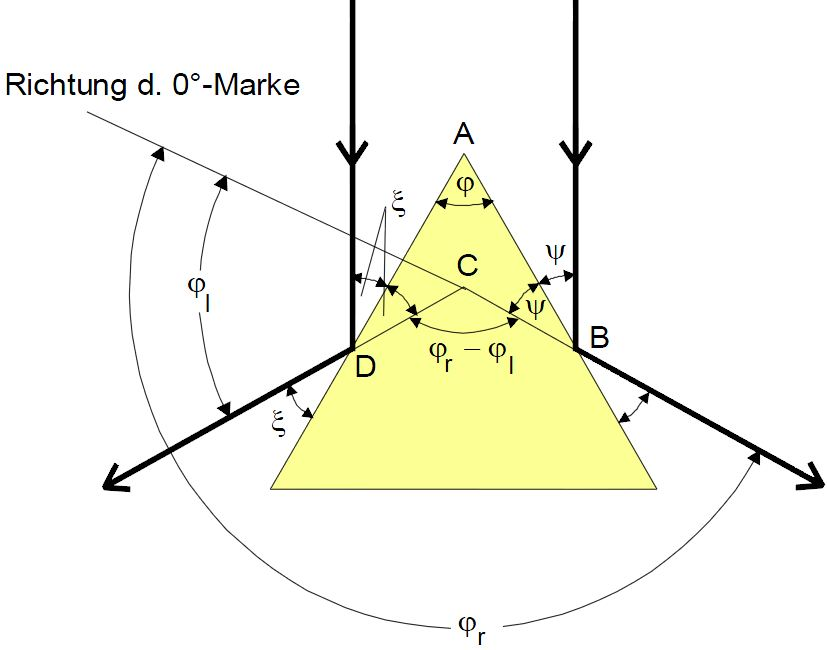
\includegraphics[scale=0.3]{picprismawinkel.jpg}
		\caption{Bestimmung des Winkels zwischen den brechenden Oberflächen[1]}
		\label{picprismawinkel}
		\end{center}	
	\end{figure}
Wird das Prisma wie in Abbildung \ref{picprismawinkel} ausgerichtet, kann aus einfachen
Winkelbeziehungen durch Messen der Reflektionswinkel beider Lichtstrahlen der brechende 
Winkel $\phi$ des Prismas bestimmt werden.
\begin{align}
\phi&=\frac{1}{2}(\phi_r - \phi_l)
\end{align}
\subsection{Bestimmung der Brechungswinkel der Spektrallinien}
	\begin{figure}[h]
		\begin{center}
		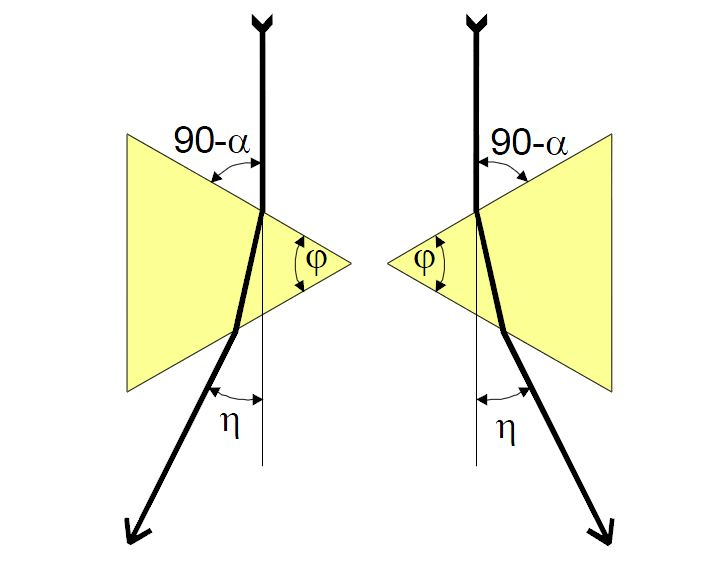
\includegraphics[scale=0.3]{picbrechwinkel.jpg}
		\caption{Brechwinkelbestimmung mit spiegelbildlicher Prismenstellung[1]}
		\label{picbrechwinkel}
		\end{center}	
	\end{figure}
Aus zwei zueinander spiegelsymmetrischen Stellungen des Prismas können die Brechungswinkel
bestimmt werden. Bei dem Zusammenfallen der gebrochenen Lichtstrahlen mit dem reflektierten
Lichtstrahl lässt sich mit Abbildung \ref{picbrechwinkel} folgende Beziehung ableiten.
\begin{align}
\eta&=180-(\Omega_r-\Omega_l)
\end{align}